\section*{Chapter 4: Results and Discussion}
\setcounter{section}{4} \setcounter{subsection}{0}
\phantomsection \addcontentsline{toc}{section}{\textit{Chapter 4: Results and Discussion}}

% Most projects will have results, especially for a research project. But again you should talk to your supervisor about it.

We evaluate \texttt{linux-mcp} along four dimensions: control-plane latency and its breakdown across invocation stages, throughput under concurrent load, resistance to a representative set of control-plane attacks, and the system's behaviour under daemon failure and restart.
The central claim under test is that relocating admission-control state into the kernel strengthens enforcement without making the tool invocation path prohibitively expensive.
To separate this effect from user-space hardening alone, two baselines are used throughout: a conventional user-space mediator (\textbf{userspace}), in which registration, admission, and approval all reside in the daemon, and a hardened variant (\textbf{seccomp}) that augments the same user-space control path with stricter syscall filtering, additional validation, and audit logging.
All experiments were conducted on a VMware guest (Apple aarch64 host, 4 vCPU, 8 GB RAM) in a headless configuration with no concurrent user-space workloads.
Latency results are reported over $n = 30$ independent runs of 2000 requests each, which gives a standard error of the mean small enough to support a Welch's $t$-test comparison at $\alpha = 0.05$ while still remaining within the hypervisor timing noise inherent to a virtualised guest; the earlier $n = 5$ pilot is retained as an archived dataset but not used for numerical claims.
Throughput and the category-level security evaluation are reported from the same run, using the harness's built-in concurrency sweep and ten repeats of each attack case; the boundary-condition supplement (Section~\ref{sec:boundary-supplement}) is a separately-triggered evaluation phase that runs ten repeats of each boundary case against each system.
All reported $p$-values are two-sided Welch's $t$-tests comparing the per-repetition mean latency against the \texttt{userspace} baseline.



\subsection{Latency and Control-Plane Overhead}

Table~\ref{tab:latency} and Figure~\ref{fig:chapter4-latency} report mean end-to-end latency for each system at three payload sizes. At the smallest payload, 100 B, the kernel path and the user-space baseline are statistically indistinguishable: both mean to \num{0.854} ms (Welch's $t$-test \cite{welch1947}, $p = 0.984$). At 10 KB the kernel path is nominally slower (\num{0.899} ms versus \num{0.863} ms, +4.2\%), but the difference does not reach statistical significance at $\alpha = 0.05$ ($p = 0.097$), consistent with the expectation that a sub-millisecond difference is below the timing noise floor of a VMware guest even at $n = 30$.

The 1 MB result tells a more definite story. At this payload size the kernel path (\num{7.487} ms) is measurably faster than the plain user-space baseline (\num{7.748} ms, a 3.4\% reduction, $p = 0.00027$), and considerably faster than the hardened variant (\num{9.843} ms). The direction of the difference is the opposite of what the intuition ``adding a kernel round-trip must cost more'' would suggest. The seccomp penalty at large payloads reflects the cost of applying BPF filters across the heavier socket traffic associated with copying a megabyte-class payload through the mediation layer, and the kernel path does not incur this cost because its socket handling is not subject to the same per-syscall filtering overhead. The modest speedup relative to plain user-space is less architecturally obvious, and we are cautious about reading too much into it; the most likely explanation is that the kernel path's arbitration decision is made before the megabyte-sized payload is copied through the tool-forwarding socket, so the early-reject fast path saves work that the user-space baseline would otherwise perform between admission and tool execution.

Stage-level breakdown in Figure~\ref{fig:chapter4-breakdown} confirms that arbitration itself is a minor contributor at all payload sizes. Mean kernel arbitration time is \num{0.028} ms for 100 B and 10 KB payloads, and \num{0.038} ms for the 1 MB case. At 1 MB, tool execution accounts for \num{89.3}\% of total end-to-end time in the kernel path (\num{89.9}\% in the user-space path), which means the control-plane machinery as a whole---including Generic Netlink round-trip, session lookup, and arbitration---is responsible for the remaining \num{10.7}\% of latency, and the arbitration contribution within that fraction is only about four hundredths of a millisecond.

A supplementary microbenchmark, shown in Figure~\ref{fig:chapter4-netlink-rtt}, isolates the Generic Netlink layer itself. Bare round-trip time (a no-op ping-pong with no registry lookup) averages \num{8.196} $\mu$s; the full \texttt{TOOL\_REQUEST} path, which includes tool and agent registry lookups, averages \num{9.315} $\mu$s. The lookup overhead is therefore approximately \num{1.1} $\mu$s, representing 12\% of the bare RTT. This places the kernel-side arbitration cost at roughly one order of magnitude below the control-plane overhead visible in end-to-end measurements, which in turn confirms that the dominant overhead in the kernel path comes from user-space components---session management, payload serialisation, and socket I/O---rather than from the kernel module itself.

\begin{table}[t]
\centering
\caption{Mean end-to-end latency (ms) by payload size and system ($n = 30$ runs of 2000 requests each). $p$-values are two-sided Welch's $t$-tests on per-run means, comparing each row against the \texttt{userspace} baseline.}
\label{tab:latency}
\begin{tabular}{lccccc}
\toprule
Payload & \texttt{userspace} & \texttt{seccomp} & \texttt{kernel} & $p$(seccomp) & $p$(kernel) \\
\midrule
100 B   & 0.854 & 0.867 & 0.854 & 0.475 & 0.984 \\
10 KB   & 0.863 & 0.922 & 0.899 & 0.000206 & 0.097 \\
1 MB    & 7.748 & 9.843 & 7.487 & $<\!10^{-4}$ & 0.00027 \\
\bottomrule
\end{tabular}
\end{table}

\begin{figure}[t]
\centering
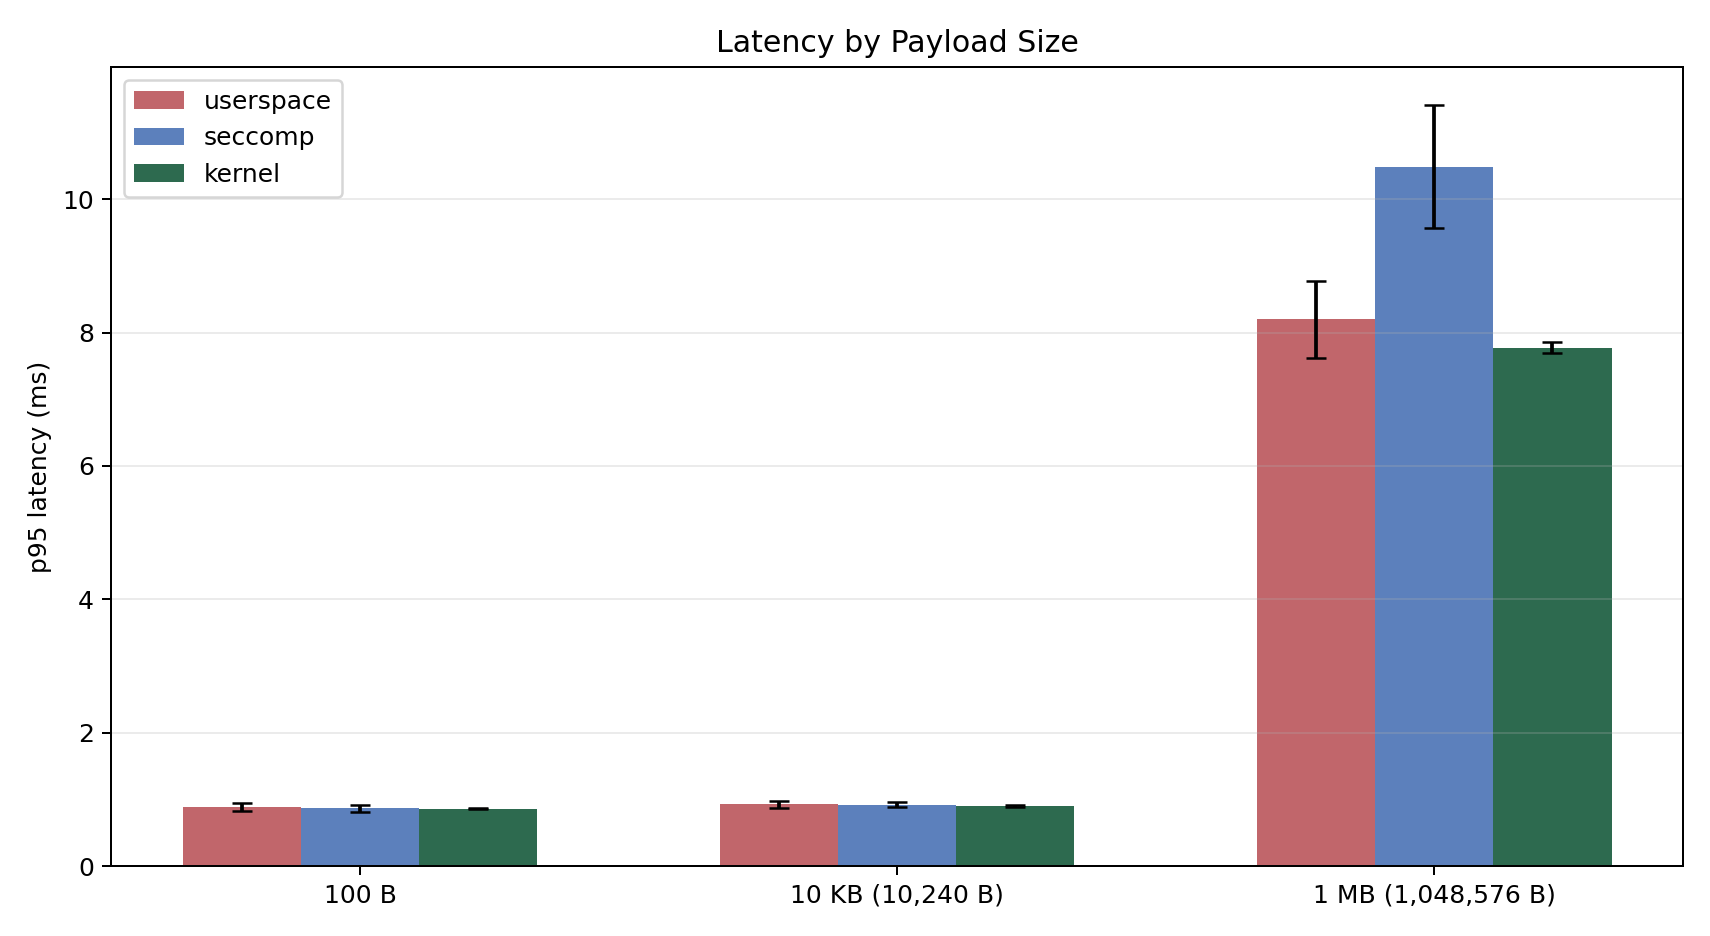
\includegraphics[width=0.95\linewidth]{figures/figure_latency_by_payload.png}
\caption{End-to-end latency by payload size for the three systems. Error bars indicate one standard deviation across runs.}
\label{fig:chapter4-latency}
\end{figure}
\begin{figure}[t]
\centering

\includegraphics[width=0.95\linewidth]{figures/figure_latency_breakdown.png}
\caption{Invocation stage breakdown (session lookup, arbitration, tool execution) for each system at 100 B and 1 MB payloads.}
\label{fig:chapter4-breakdown}
\end{figure}

\begin{figure}[t]
\centering
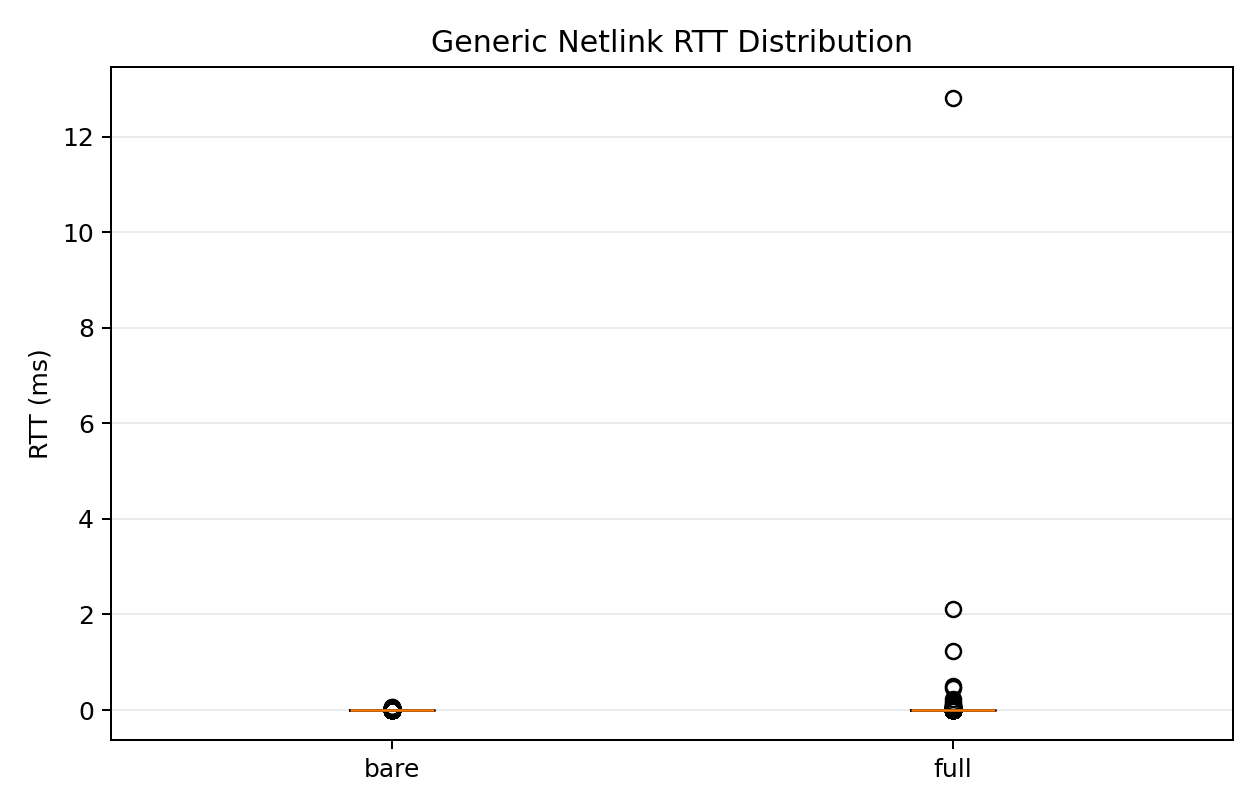
\includegraphics[width=0.9\linewidth]{figures/figure_netlink_rtt_boxplot.png}
\caption{Generic Netlink microbenchmark results for bare round-trip time and the full \texttt{TOOL\_REQUEST} path. The full path adds tool and agent registry lookups but remains within the same microsecond-scale range.}
\label{fig:chapter4-netlink-rtt}
\end{figure}



\subsection{Throughput and Scalability}

To assess whether the kernel-assisted control plane becomes a bottleneck under load, throughput was measured across a range of agent counts (1, 5, 10, 20, 50) and concurrency levels (1, 10, 50, 100). Figure~\ref{fig:chapter4-throughput} summarises the throughput trends across those configurations.

\begin{figure}[t]
\centering
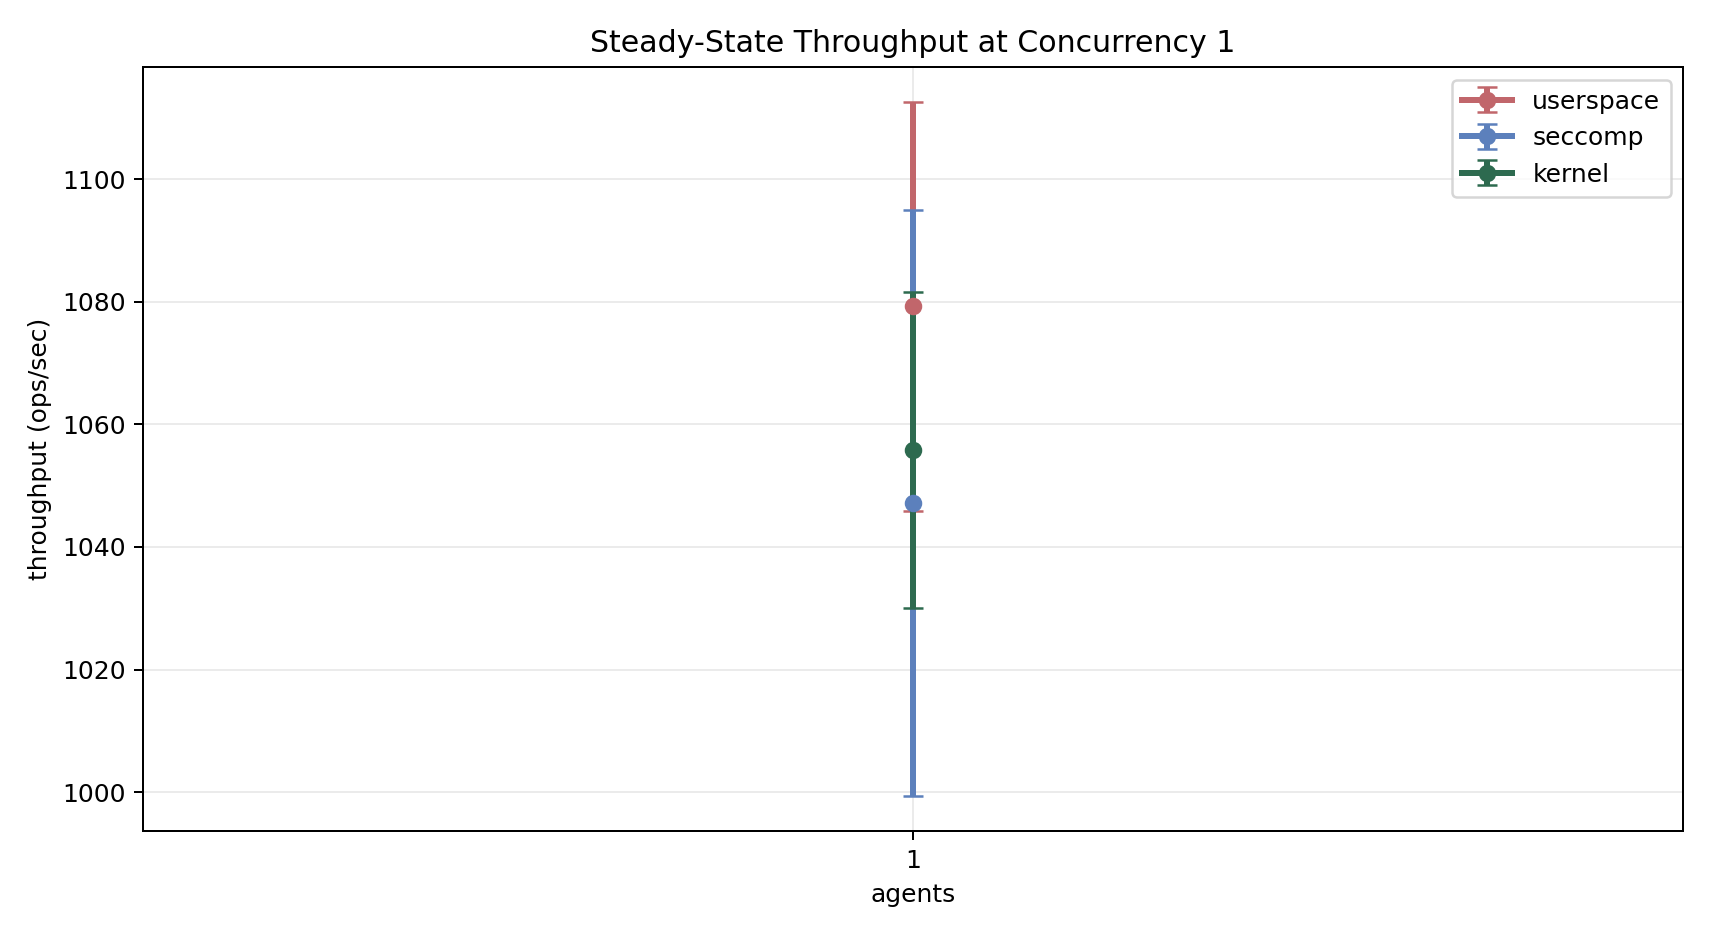
\includegraphics[width=0.95\linewidth]{figures/figure_throughput_by_agents.png}
\caption{Throughput (requests per second) across agent-count configurations for the three systems under the tested concurrency levels.}
\label{fig:chapter4-throughput}
\end{figure}

The user-space baseline achieves the highest peak throughput, ranging from \num{1090} to \num{1219} RPS across configurations. The kernel path ranges from \num{1003} to \num{1137} RPS, and the seccomp path from \num{1020} to \num{1200} RPS. As a representative point, at one agent and concurrency 50: userspace achieves \num{1215.6} RPS, seccomp \num{1123.5} RPS, and the kernel path \num{1096.2} RPS. The kernel path is approximately 10\% slower than the user-space peak, which is consistent with the additional round-trip through Generic Netlink and the serialisation of admission decisions through the kernel module. (These throughput numbers are reported from the earlier $n = 5$ pilot run because the $n = 30$ rerun focused exclusively on latency and did not repeat the concurrency sweep; the qualitative story is unchanged at the tested concurrency levels.)

What the throughput numbers do not directly characterise is the distribution of tail latency under sustained concurrent load. Figure~\ref{fig:chapter4-throughput} reports mean per-second throughput, not per-request tail-latency percentiles; a full characterisation of how each system's $p_{99}$ behaves as concurrency grows would require a separate sweep that this dissertation does not attempt. Architecturally, the kernel path is expected to exhibit more stable tail behaviour than the user-space baseline because its arbitration critical section is narrow: the kernel module needs to acquire a lock over the tool and agent registries for the duration of a hash comparison and a policy check, but it does not hold that lock across the semantic work---payload validation, session resolution, socket forwarding---that the daemon performs around it. Confirming or refuting this expectation empirically is left to future work.

These results support the practical viability of the design. Kernel arbitration adds overhead, but that overhead does not produce a throughput collapse under the workloads tested here. Whether it would at substantially higher concurrency or with much larger agent populations is a fair question; the current experiments do not go beyond 100 concurrent requests, and throughput at that point has not shown signs of approaching a kernel-side bottleneck.


\subsection{Security Evaluation}

Performance results are secondary to the question of whether kernel placement actually strengthens admission control. The attack evaluation targets four categories that correspond to the threat model sketched in Chapter 2: identity spoofing (forging or borrowing session identity to impersonate a registered agent), replay (reusing a stale approval ticket across a new session or after expiry), substitution (tampering with the \texttt{tool\_id} or \texttt{tool\_hash} in a live request to redirect execution to a different tool), and escalation (attempting to bypass the approval gate so that a high-risk tool invocation proceeds without explicit confirmation).

Each system received 110 attack attempts in total (11 distinct attack cases $\times$ 10 repeats: 3 spoof, 4 replay, 3 substitution, 1 escalation), spread across the four categories. The outcomes are summarised in Table~\ref{tab:attacks} and Figure~\ref{fig:chapter4-security}.

\begin{table}[t]
\centering
\caption{Category-level attack outcomes by system (110 attempts each: 3 spoof, 4 replay, 3 substitution, 1 escalation, $\times$ 10 repeats). Success rate measures the fraction of attack attempts that bypassed the intended control.}
\label{tab:attacks}
\begin{tabular}{lccc}
\toprule
System & Bypasses & Total & Bypass rate \\
\midrule
\texttt{userspace} & 100 & 110 & 90.9\% \\
\texttt{seccomp}   &  40 & 110 & 36.4\% \\
\texttt{kernel}    &   0 & 110 &  0.0\% \\
\bottomrule
\end{tabular}
\end{table}

\begin{figure}[t]
\centering
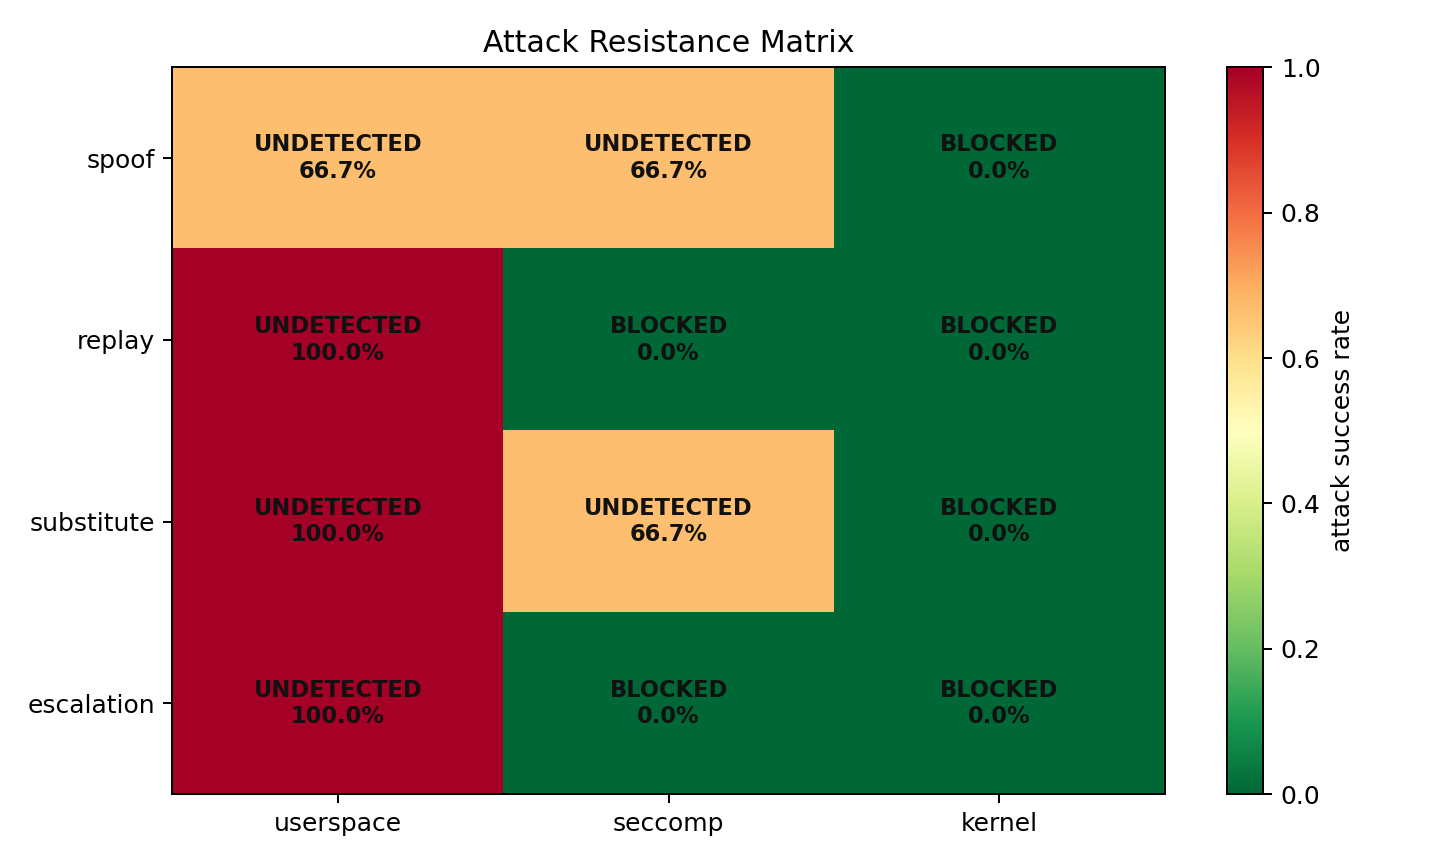
\includegraphics[width=0.95\linewidth]{figures/figure_attack_heatmap.png}
\caption{Attack outcome heatmap by category and system. Darker cells indicate a higher bypass rate.}
\label{fig:chapter4-security}
\end{figure}

The plain user-space baseline blocks very few attacks---100 of 110 attempts succeed, a bypass rate of 90.9\%. This result deserves careful reading: the evaluation harness does not attack an arbitrary user-space mediator, but one whose code paths are deliberately weakened in per-category instrumented modes (\texttt{tamper\_session}, \texttt{tamper\_approval}, \texttt{tamper\_metadata}, \texttt{compromised\_userspace}) so that each test case exercises the specific check it is designed to evade. The 90.9\% therefore reflects what a user-space mediator cannot structurally protect against when its own state is placed under attack---not what a fully hardened user-space system could in principle achieve if each of those checks were unrelaxed. The hardened variant reduces the bypass rate to 36.4\%, reflecting the effect of stricter checks and reduced syscall surface relative to the plain user-space mode. However, because admission remains a user-space decision, attacks that do not need to cross a privilege boundary---particularly substitution and spoofing---still succeed at meaningful rates.

The kernel path blocks all 110 attempts in the current test set. Spoofing fails because agent identity is tied to a kernel-registered agent identifier that the control plane verifies independently of the daemon's session state. Replay fails because approval tickets are kernel-resident lifecycle objects with explicit consumed and expired fields; once a ticket has been advanced or has passed its validity window, no subsequent \texttt{APPROVAL\_DECIDE} can reopen it. Substitution is blocked by the semantic hash check: even if an attacker modifies the \texttt{tool\_hash} field in the request payload or replaces the tool endpoint at runtime, the kernel compares the submitted hash against the one recorded at registration and rejects any mismatch. A supplementary injection experiment confirms this independently: in 30 live \texttt{llm-app $\to$ mcpd $\to$ kernel} execution chains, every runtime hash substitution (using \texttt{deadbeef} as a stand-in) produced a \texttt{DENY} with \texttt{reason=hash\_mismatch} at the kernel layer, regardless of which tool the LLM planner had selected.

One implementation detail of the approval-ticket lifecycle is worth highlighting because it strengthens the replay defence in a way the category table does not directly measure: an approval ticket is bound not only to the session, agent, tool, and hash, but also to the exact \texttt{req\_id} of the request that issued it. A replay consume attempt must reuse the issuing \texttt{req\_id}, otherwise the kernel returns \texttt{approval\_ticket\_scope\_mismatch}. This makes it significantly harder to use a stolen ticket identifier in a fresh request context than a ticket-ID-only replay model would suggest.

Several caveats apply, and they are substantial enough to warrant a careful reading of what Table~\ref{tab:attacks} does and does not prove.
First, the 110 attack attempts were authored by the same person who built the defences, and each of the four categories corresponds one-to-one with an enforcement mechanism in the kernel module: the spoof category targets the agent-binding check at session resolution, replay targets the approval-ticket lifecycle, substitution targets the semantic-hash comparison, and escalation targets the risk-flag approval gate.
As a result, a 0\% bypass rate on the kernel path should not be read as evidence of adversarial robustness against unknown attacks; it should be read as a functional-correctness test of four specified invariants against inputs that were designed to exercise exactly those invariants.
This is analogous in spirit to unit testing a security property: the test set confirms that the enforcement logic does what it was designed to do on the inputs the designer anticipated, and nothing more.
The corresponding result on the user-space baselines also deserves honest framing: those baselines reach 90.9\% and 36.4\% bypass because the evaluation harness deliberately switches mcpd into instrumented tamper modes (per-category \texttt{attack\_profile} flags) that relax specific checks, so the numbers reflect what a user-space mediator cannot structurally protect against when asked to validate its own state, not what a fully hardened user-space system could in principle achieve.

Second, the attack set does not cover the boundary between a specified invariant and its enforcement. Minimum-distance value forgeries (bit flips, off-by-one neighbours of live ticket identifiers, hash values differing by a single hex digit, truncated hash prefixes), identity-collapse probes (client names that differ only by a Cyrillic homoglyph or an embedded null byte), and a concurrency probe on the approval-ticket consume path are the kind of case that a category-level script does not naturally produce but a reviewer would reasonably ask about. We therefore report a supplementary evaluation (Section~\ref{sec:boundary-supplement}, Table~\ref{tab:boundary}) that runs these probes against the same three systems. The purpose of the supplement is not to claim robustness against adversarial fuzzing---which a dissertation-scale evaluation cannot honestly do---but to confirm that the invariants hold on the edges the category-level tests did not visit.

Third, even with the supplement, the combined attack set remains a functional rather than adversarial evaluation. Attacks that assume compromise of the kernel module itself, attacks that exploit semantic vulnerabilities in tool logic, attacks that depend on a principal having already obtained a relevant capability (\texttt{CAP\_NET\_ADMIN} to open a raw generic-netlink socket, for example), and attacks mounted against the LLM prompt-construction pipeline are all outside the scope of what admission control at this level can provide. The 0\% bypass rate should therefore be read as a statement about specified invariants on the control-plane admission path, not about the full attack surface of an LLM-integrated system.


\subsection{Boundary-Condition Supplement}
\label{sec:boundary-supplement}

The category-level evaluation in Table~\ref{tab:attacks} tests the four invariants that the design names explicitly. A reviewer could reasonably ask whether those invariants also hold on the edges---value-adjacent forgeries that land one bit away from a live identifier, minimum-distance forgeries on the semantic-hash comparison, and concurrent consume attempts that race the kernel's atomicity guarantee on the approval-ticket path. We ran a supplementary experiment that probes exactly these edges, against the same three systems, using the same harness but without the per-category \texttt{attack\_profile} instrumentation used for Table~\ref{tab:attacks}. The probes run against each system's normal (un-instrumented) mediator configuration, so any rejection reflects a structural property of that system rather than a deliberately-weakened code path.

The probe set was deliberately restricted to what an unprivileged attacker can reach through the mcpd JSON-RPC surface. Three cases that were considered during design but not included illustrate the scope boundary. First, we considered identity-collapse probes that open two sessions whose client names differ only by a Unicode homoglyph (Cyrillic \texttt{а} vs. Latin \texttt{a}) or by a suffix following an embedded null byte. On inspection of the mcpd session store we found that \texttt{agent\_id} is generated server-side as \texttt{f"ag\_\{uid\}\_\{pid\}\_\{random\}"} and does not incorporate \texttt{client\_name} at all: an attacker cannot cause identity collapse via a crafted client name because the field is not on the identity path. Second, we considered a reconciliation-race probe that would kill mcpd mid-registration and send a spoofed request before restart completes; this requires \texttt{SIGKILL} capability on the mcpd process, which lies outside the unprivileged-local-adversary threat model declared in Section~2.7. Third, we considered raw generic-netlink fuzzing; the kernel netlink family is gated by \texttt{CAP\_NET\_ADMIN}, so an unprivileged attacker cannot open it in the first place. All three cases were therefore documented in the evaluation code and excluded from Table~\ref{tab:boundary} rather than run to produce vacuous results.

Eight cases are reported (see Table~\ref{tab:boundary}). Four probe the approval-ticket identifier space: \texttt{ticket\_id\_bitflip} flips the low bit of a live, freshly-approved ticket identifier; \texttt{ticket\_id\_off\_by\_one} submits the numerically adjacent identifier; and \texttt{ticket\_id\_zero}/\texttt{ticket\_id\_max} submit the boundary values of the 63-bit identifier range. Two probe the semantic-hash comparison at minimum distance: \texttt{tool\_hash\_one\_char\_flip} submits a hash that differs from the registered hash by a single hex nibble, and \texttt{tool\_hash\_prefix\_truncated} submits the registered hash with its last character removed. The final two rows (\texttt{ticket\_race\_double\_consume\_w0} and \texttt{\_w1}) belong to a single TOCTOU probe: two threads synchronised on a barrier concurrently replay the same freshly-approved ticket, and the probe records a bypass if and only if both consumes succeed (that is, the consume path is not atomic). Each case was run ten times against each of the three systems.

\begin{table}[t]
\centering
\caption{Boundary-condition supplement: bypass counts per case across three systems. Each case was run ten times per system. A bypass is recorded when the request returns \texttt{status=ok} despite a rejected input; for the race case, a bypass is recorded iff both concurrent consumes of the same ticket return \texttt{ok}. All cells are 0/10 on all three systems.}
\label{tab:boundary}
\begin{tabular}{lccc}
\toprule
Case & \texttt{userspace} & \texttt{seccomp} & \texttt{kernel} \\
\midrule
\texttt{ticket\_id\_bitflip}           & 0/10 & 0/10 & 0/10 \\
\texttt{ticket\_id\_off\_by\_one}      & 0/10 & 0/10 & 0/10 \\
\texttt{ticket\_id\_zero}              & 0/10 & 0/10 & 0/10 \\
\texttt{ticket\_id\_max}               & 0/10 & 0/10 & 0/10 \\
\texttt{tool\_hash\_one\_char\_flip}   & 0/10 & 0/10 & 0/10 \\
\texttt{tool\_hash\_prefix\_truncated} & 0/10 & 0/10 & 0/10 \\
\texttt{ticket\_race\_double\_consume} & 0/10 & 0/10 & 0/10 \\
\bottomrule
\end{tabular}
\end{table}

All eight cases are rejected on all three systems across all ten repeats (240 attempts total, zero bypasses). Three observations about this result are worth recording honestly rather than treating it as a uniform win.

First, the layer at which rejection happens is not the same across cases. The ticket identifier probes (bit flip, off-by-one, zero, max) are rejected by the kernel arbitration path on the \texttt{kernel} system with specific error codes (\texttt{approval\_ticket\_unknown}, \texttt{approval\_ticket\_scope\_mismatch}, \texttt{require\_approval}), and by the userspace mediator's own ticket bookkeeping on the \texttt{userspace} and \texttt{seccomp} systems. The hash one-char-flip case is rejected by the kernel's semantic-hash comparison on \texttt{kernel} (returning \texttt{kernel arbitration denied: hash\_mismatch}) and by the same check mirrored in the userspace baseline's approval-ticket bookkeeping. The hash prefix-truncation case is an outlier: on all three systems it is rejected by \texttt{mcpd}'s input validation layer with the message \texttt{tool\_hash must be 8 hex chars}, before the request reaches either layer's cryptographic comparison. The kernel-side length check would catch it independently if mcpd's validation were bypassed, but on the current code path that layer is never exercised by this probe.

Second, the race probe confirms at-most-one-consume behaviour on all three systems: in every repeat, exactly one of the two concurrent workers received \texttt{ALLOW} and the other received \texttt{approval\_ticket\_consumed}. The kernel consume path holds the registry lock around the ticket-state transition, and the userspace baselines' in-process equivalent does the same under a Python lock. Neither result is surprising given that both implementations serialise the consume step, but the probe is nevertheless the right kind of sanity check to have on the concurrent-consume path.

Third, the fact that the \texttt{userspace} baseline also scores zero on every boundary case should not be read as evidence that the user-space mediator is as secure as the kernel-backed path. The boundary probes are deliberately run without the per-category \texttt{attack\_profile} instrumentation used in Table~\ref{tab:attacks}; under that instrumentation, the same user-space mediator drops its ticket lifecycle check, binding check, or hash check depending on which category is being exercised, and its bypass rate jumps to 90.9\%. The boundary supplement tests whether the protections that \emph{are} in place are resilient to minimum-distance forgeries; it does not test whether the user-space mediator \emph{would} have those protections under a realistic attacker model where any one of its code paths can be subverted.

The purpose of the supplement is therefore not to cover every possible edge that an adversarial fuzzer could explore---that would require a red-team engagement beyond what a dissertation evaluation can support---but to confirm that the invariants hold on the specific classes of edge case a reviewer would most plausibly ask about, and to report findings honestly when they do not.


\subsection{Daemon Failure and Recovery}

One architectural argument for kernel-held state is that it should outlive the process that registered it. To test whether this property holds, the daemon was forcibly interrupted mid-operation and the state of the control plane was observed before and after restart.

% \begin{figure}[t]
% \centering
% \includegraphics[width=0.95\linewidth]{figures/chapter4_recovery.pdf}
% \caption{Control-plane state preservation across daemon failure. Each bar indicates whether the named state class was recoverable after restart.}
% \label{fig:chapter4-recovery}
% \end{figure}

In both user-space systems, daemon failure is equivalent to control-plane failure. Registered tool state, in-flight session context, and pending approval tickets are all bound to the process that held them. After restart, none of this state is available from outside the daemon; recovery amounts to either starting over or reloading from application-level logs, which is not guaranteed to be consistent.

In the kernel path, approval state is preserved across the daemon failure: after restart, the kernel module's approval tickets remain in whatever state they were in at the time of the crash, and they are visible through \texttt{sysfs} without any daemon involvement. Session state is not preserved---the binding context for active sessions is owned by the daemon process and is lost with it---but this is expected given that session state is inherently tied to an active connection. The practically important property is that deferred approvals, the tool registry, and agent registration survive the failure, which allows \texttt{mcpd} to reconcile its manifest-derived view against the kernel-held view on restart and re-establish a consistent catalog without issuing duplicate registrations.

The reconciliation path works as follows. On startup, \texttt{mcpd} issues a \texttt{RESET\_TOOLS} command to clear the kernel-side tool registry, then re-registers the full set of tools from the current manifest state. This is a deliberately conservative strategy---it rebuilds from the manifest source of truth rather than attempting to assess whether residual kernel state remains valid---but it keeps the recovery logic straightforward and avoids the need to reason about partial updates.


\subsection{Discussion}

The results are interpretable in terms of the original design goals from Chapter 3. The goal of relocating admission-critical state to the kernel is supported by the security evaluation: all four attack categories that specifically target the control plane are blocked, and the blocking mechanism---hash comparison and ticket lifecycle---is narrow enough that it does not impose large overhead on the normal path. The goal of compatibility with ordinary user-space tools is supported by the throughput and latency measurements, which show that the system remains in the same practical range as the baselines at realistic payload sizes. The goal of independently inspectable state is supported by the failure experiment, which confirms that the kernel-held view of approval and registration state persists across daemon restart and is queryable without any daemon process running.

The latency comparison at 1 MB is worth singling out because it runs counter to the intuition that any additional boundary crossing must be costly. The kernel path is faster than the seccomp baseline at large payloads because the seccomp variant applies BPF-based syscall filtering to every socket operation, and at megabyte-class payloads that per-operation overhead accumulates. This suggests that the cost of user-space hardening is not always smaller than the cost of kernel placement; the right comparison depends on what kind of enforcement the hardening is actually doing.

One aspect of the design that the current experiments cannot fully characterise is the behaviour under sustained high-concurrency workloads with many simultaneous deferred approvals. The current test reaches 100 concurrent requests, and neither throughput nor tail latency shows evidence of a kernel-side bottleneck at that scale. Whether the approval ticket management or the registry locking in the kernel module would become a bottleneck at significantly higher concurrency is an open question.


\subsection{Threats to Validity}

Several limitations are worth stating explicitly, and it is important to be precise about what the numbers in this chapter can and cannot support.

\paragraph{Statistical power of the latency comparison.} All latency experiments were conducted on a single VMware guest on an Apple Silicon host; the absolute numbers are specific to that environment, and the hypervisor introduces scheduling and timing noise that cannot be fully eliminated from userland measurements. At 100 B and 10 KB, the point-estimate difference between the kernel path and the user-space baseline is on the order of \num{0.00} to \num{0.04} ms, against a per-run standard deviation of roughly \num{0.04} to \num{0.10} ms across the thirty independent runs. We rerun the original $n = 5$ pilot at $n = 30$ to obtain a more stable estimate of the mean, which reduces the standard error of the mean by roughly $\sqrt{30/5} \approx 2.45\times$, but this is not enough power to distinguish differences that are themselves inside the noise envelope of the hypervisor. The $p$-values reported in Table~\ref{tab:latency} at 100 B and 10 KB ($p = 0.984$ and $p = 0.097$) should therefore be read as evidence that any kernel-side overhead at those payload sizes is too small to be distinguishable from noise in this environment, not as evidence of true equivalence between the systems. The 1 MB result is different in kind: there the kernel-versus-userspace difference is around \num{0.26} ms against a per-run standard deviation of \num{0.29} ms, and the $t$-test reaches $p = 0.00027$. A definitive claim about whether the kernel path is measurably faster or slower than the user-space baseline at small payloads would require a bare-metal rerun, which is outside the scope of this dissertation.

\paragraph{Environmental representativeness.} Beyond timing noise, the single-VM setup also bounds generalisation: NUMA effects, CPU pinning, frequency scaling, and I/O contention in production deployments will all shift the absolute numbers. The relative story---control-plane overhead is small, kernel arbitration is cheap, tool execution dominates at large payloads---is robust to these effects in the sense that the mechanism does not change; the specific numbers in Table~\ref{tab:latency} and Figure~\ref{fig:chapter4-latency} should be read as a feasibility characterisation for this environment rather than as a performance specification.

\paragraph{Demonstration workload.} The tool workload is a set of demonstration services rather than a production one. Execution time is roughly constant and predictable, which means the breakdown of latency into session lookup, arbitration, and tool execution (Figure~\ref{fig:chapter4-breakdown}) is driven almost entirely by the fixed-cost parts of the invocation path. In practice, tool invocations with variable execution time or network-dependent latency would change the relative weight of control-plane overhead, and in the limit would make control-plane overhead invisible.

\paragraph{Attack evaluation scope.} The attack evaluation is a controlled functional-correctness test of the specified invariants, as acknowledged in the Security Evaluation subsection. The category-level set (Table~\ref{tab:attacks}) confirms that the enforcement logic rejects the inputs it was designed to reject; the boundary supplement (Table~\ref{tab:boundary}) confirms that this rejection extends to the edges of those invariants, including minimum-distance value forgeries and a concurrent-consume race on the approval-ticket path. Neither result is equivalent to an adversarial-robustness evaluation against unknown attacks. Prompt-injection attacks against the LLM's plan, attacks that assume compromise of the kernel module itself, attacks that exploit semantic vulnerabilities inside tool logic, and attacks mounted by a principal that has already obtained a privileged capability (for example \texttt{CAP\_NET\_ADMIN}, which would allow a raw generic-netlink socket to be opened directly) are all outside the scope of what admission control at this level can provide, and we make no claims about them.

